\documentclass[twoside,colorback,accentcolor=tud4c,11pt]{tudreport}
\usepackage{ngerman}
\usepackage[utf8]{inputenc} 
\usepackage[T1]{fontenc}
\usepackage{siunitx}
\usepackage{hyperref}
\usepackage{units}
\usepackage{upgreek}
\usepackage{biblatex}
\usepackage{graphicx}
\usepackage{float}
\usepackage{subfigure}
\usepackage[figure]{hypcap}
\usepackage{amsmath}
\usepackage{cancel}
\usepackage{braket}

\title{Nd:YAG}
\subtitle{	\begin{tabular}{p{8cm}ll}
Benedikt Paul Schallmo   &   Dominik Pfeiffer \\ Matrikelnummer: 2686286  &   Matrikelnummer: 2913632       \\ email: \textaccent{ benediktschallmo@yahoo.de} & email: \textaccent{dominik@diepfeiffers.de}  
			\end{tabular} }
\subsubtitle{ \\Versuchsbetreuung : Dr. Matthias Sinther \\ Datum der Durchführung: 22.05.2027 \\ Abgabetermin: 12.06.2017    }
\institution{Institut für Angewandte Physik}
\sponsor{Hiermit erklären wir, dass wir die vorliegende Arbeit bzw. Leistung eigenständig, ohne fremde Hilfe und nur unter Verwendung der angegebenen Hilfsmittel angefertigt haben. Alle übernommenen Textstellen aus der Literatur beziehungsweise dem Internet sind als solche kenntlich gemacht. Diese Arbeit hat in gleicher oder ähnlicher Form noch keiner Prüfungsbehörde vorgelegen. \\\\ 
\begin{tabular}{lp{2em}lp{2em}l}
 \hspace{4cm}   && \hspace{4cm}  && \hspace{4cm}
 \\\cline{1-1}\cline{3-3}\cline{5-5}
 Ort, Datum     && Benedikt Schallmo && Dominik Pfeiffer
\end{tabular}  }


\dedication{}
\lowertitleback{}
\listfiles
    
\begin{document}

\maketitle 

\tableofcontents


\chapter{Einleitung und Ziel des Versuchs}
Ziel dieses Versuches ist es, die physikalischen Eigenschaften eines Halbleiterlasers und eines Festkörperlasers zu untersuchen. Hierfür soll zunächst das Verhalten des zum Pumpen verwendeten Halbleiterlasers näher betrachtet und dessen Kennlinie bezüglich Licht-/Pumpleistung aufgenommen werden. Anschließend wird der durch diesen Halbleiterlaser gepumpte Nd:YAG-Laser näher untersucht und die optimalen Arbeitskonfigurationen herausgearbeitet um zuletzt mittels eines KTP-Kristalls das Phänomen der Frequenzverdopplung zu nutzen und einige Kenngrößen dieser zu bestimmen.
\chapter{Physikalische Grundlagen}
In folgendem Abschnitt sollen die zur Durchführung des Versuches notwendigen physikalischen Grundlagen kurz erläutert werden. Hierzu zählen vor Allem die Prozesse in Lasern als auch in der nichtlineare Optik.
\section{Grundlagen Laser}
\subsection{Laser allgemein}
Das Akronym  \textbf{LASER} steht für "'\textbf{L}ight \textbf{A}mplification by \textbf{S}timulated \textbf{E}mission of \textbf{R}adiation"`, zu deutsch: "'Lichtverstärkung durch induzierte Emission von Strahlung"` und weist bereits auf das Funktionsprinzip des Lasers hin. Durch die Absorption von Energie aus Stößen mit anderen Atomen oder elektromagnetischer Strahlung können in Atomen Elektronen auf höhere Energieniveaus gehoben werden. Durch den Übergang in ihren Grundzustand wird die Energiedifferenz der Niveaus in der Form elektromagnetischer Strahlung freigesetzt. Bei freien Atomen geschieht dies spontan und isotrop in den Raum, wobei sowohl Phase als auch Polarität des ausgesendeten Photons zufällig sind.\\
Das Konzept der stimulierten Emission wurde zuerst von A. Einstein beschrieben, ca. 44 Jahre vor der Entwicklung des ersten Lasers (1960). Hierbei wird ein angeregtes Atom in ein geeignet gewähltes elektromagnetisches Strahlungsfeld eingebracht und so zur Emission eines dem stimulierenden Photon in Phase und Polarität übereinstimmenden Photons gebracht. Um nun über diesen Prozess das Strahlungsfeld zu verstärken, muss eine s.g. Besetzungsinversion erreicht werden. Damit ist gemeint, dass sich mehr Atome im angeregten Zustand befinden müssen als im Grundzustand. Nach der Stefan-Boltzman-Verteilung ist aber der energetisch niedrigere Grundzustand im thermischen Gleichgewicht überwiegend besetzt und das Strahlungsfeld wird nicht verstärkt oder sogar abgeschwächt. Eine Besetzungsinversion ist in einem Zwei-Niveau-System (Grundzustand und ein angeregter Zustand) so instabil, dass verwendete Laser mindesten ein Drei-Niveau-System, wenn nicht sogar ein höheres Mehr-Niveau-System aufweisen \cite{prot1}.\\
Der im Laufe des Versuches aufzubauende Nd:YAG-Laser arbeitet mit einem 4-Niveau-System.
\begin{figure}[H]
\centering
   	\begin{minipage}[b]{0.8\textwidth}
   	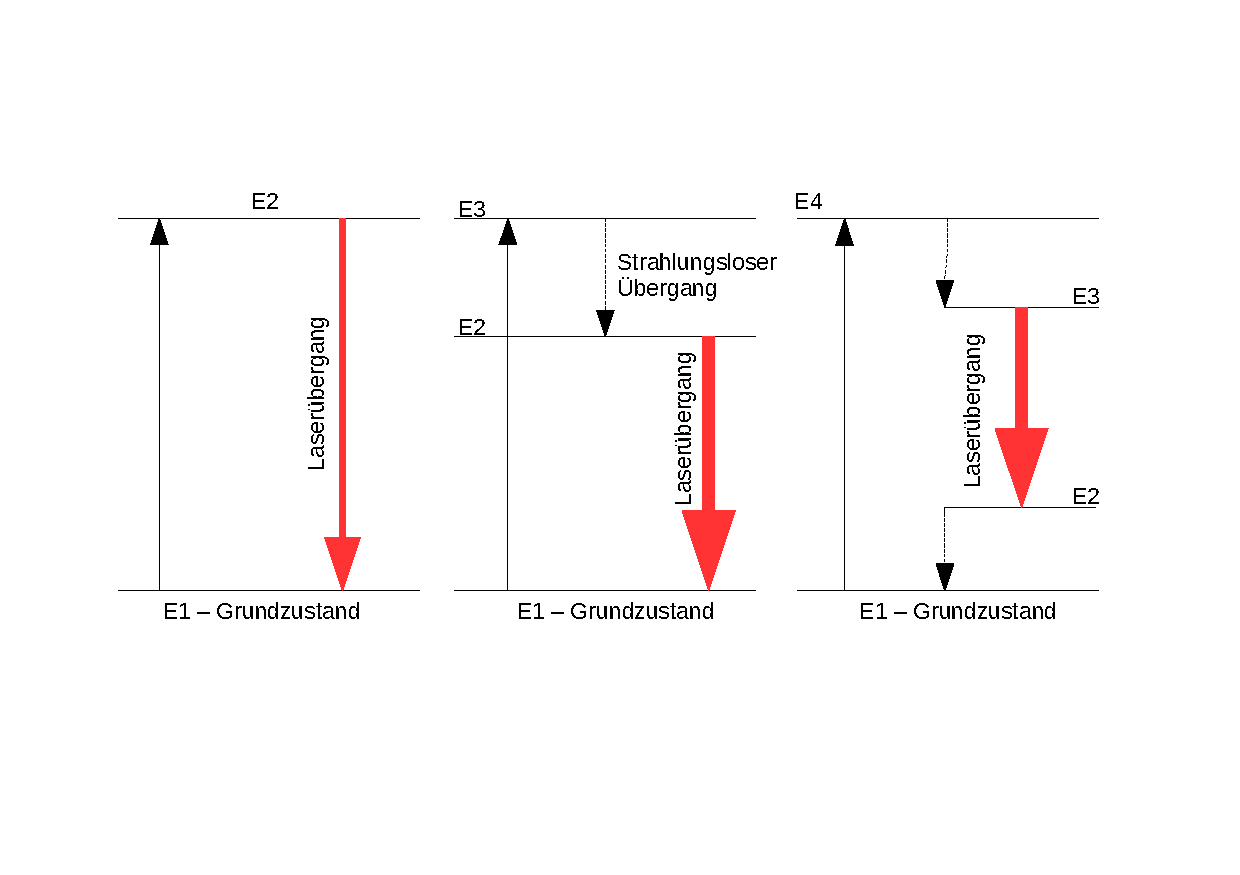
\includegraphics[width=\textwidth]{graphics/Lasersys.pdf}
  	\label{lasys}
   	\end{minipage}
\caption{Schematische Darstellung von Zwei-, Drei- und Vier-Niveau-Lasersystemen} 	
\end{figure}
\subsection{Halbleiter-Laser}
Kurz nach der Entwicklung der ersten Laser um 1960, entdeckte man auch in Halbleiterdioden Lasertätigkeit. Zunächst konnten Halbleiterlaser jedoch nur gepulst und bei geringen Temperaturen von $T<100\,\si{K}$ betrieben werden. Ab ca. 1970 konnte ein kontinuierlicher Betrieb bei Raumtemperaturen realisiert werden. Heutzutage sind Laserdioden aus dem alltäglichen Leben kaum noch wegzudenken. Sie finden in Druckern, BluRay-Playern oder Laserpointern sowie in der Medizin flächendeckend Einsatz.\\
Halbleiterlaser (HL-Laser) bestehen in der Regel aus III/V- und II/VI-Halbleitern und deren Legierungen, wobei die Römische Zahl die Hauptgruppe der Komponenten bezeichnet. Der in diesem Versuch verwendetet HL-Laser besteht aus GaAs/AlGaAs (Galliumarsenid/Alluminiumgalliumarsenid) in einer sg. Doppelheterostruktur \ref{dophet}. Der schematische Aufbau der Laserdiode ist in \ref{diau} zu sehen:
\begin{figure}[H]
\centering
   	\begin{minipage}[b]{0.6\textwidth}
   	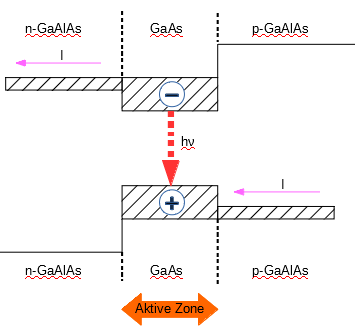
\includegraphics[width=\textwidth]{graphics/doppelhetero.PNG}
  	\label{dophet}
   	\end{minipage}
\caption{Doppelhetero-Struktur}\cite{anl}
\end{figure}
\begin{figure}[H]
\centering
   	\begin{minipage}[b]{0.6\textwidth}
   	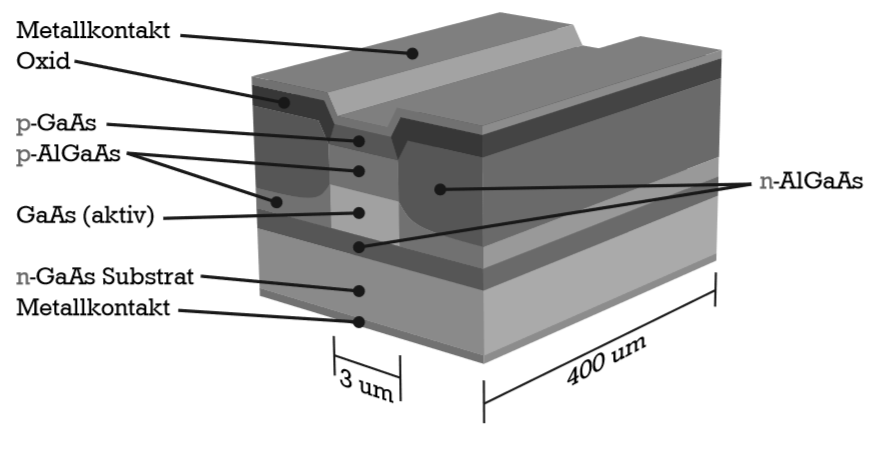
\includegraphics[width=\textwidth]{graphics/diodaufb.PNG}
  	\label{diau}
   	\end{minipage}
\caption{Aufbau der Laserdiode}\cite{anl} 	
\end{figure}
Die Besonderheit von Halbleiterlasern liegt darin, dass Aufgrund der dotierten (gewollt verunreinigten) Kristallstruktur die Energieniveaus nicht mehr in diskreter Form, sondern in quasi-kontinuierlichen Form vorliegen. In einer Halbleiterdiode werden ein p- und ein n-Dotiertes Material in Kontakt gebracht. Im so entstehenden p-n-Übergang findet der eigentliche Lasertätigkeit statt. Um die Laserbedingung, also eine Besetzungsinversion zwischen Leitungs- und Valenzband zu erreichen müssen die Energieintervalle der Bänder je zu mehr als $50\%$ mit Elektronen bzw. Löchern besetzt sein. Obwohl sich die Elektronen/Löcher innerhalb des jeweiligen Bandes zwar im thermischen Gleichgewicht befinden, gilt dies mitnichten für den Halbleiter als Ganzes. Über die Quasi-Fermi-Statistik lässt sich die Besetzungswahrscheinlichkeit f(W) der Energiezustände innerhalb der Bänder beschreiben:
\begin{equation}
f(W)=\frac{1}{1+\exp\left(W-W_{L,V}\right)/ (k_{b}T)}
\end{equation}
wobei $W_{L,V}$ die Quasi-Fermienergien des betrachteten Bandes ist. Damit ergibt sich die s.g. Bernard-Duraffourg'sche Laserbedingung zu $W_{g}<h\nu <W_{L}-W_{V}$. Bei einem HL-Laser wie dem hier verwendeten erreicht man die Besetzungsinversion über das Anlegen einer Spannung in Durchlassrichtung der Diode und den daraus resultierenden Strom. \\
Um mehr stimulierte als spontane Emission zu erzwingen, muss wie bei jedem Laser ein Resonator Teil des Aufbaus sein. Bei HL-Lasern erreicht man dies, indem der Kristall entlang einer bestimmten Achse spaltet. Aufgrund des hohen Brechungsindexes des Kristalles gegenüber der Luft erzielt man so bereits eine Reflektivität von knapp 30\%, was ausreicht um Lasertätigkeit zu ermöglichen. Um das Laserlicht in bestimmte Richtungen zu führen, bettet man das aktive Medium (GaAs), in der die Rekombination von Elektronen und Löchern stattfinden soll, oftmals in andere Materialien mit niedrigerem Brechungsindex und größerer Bandlücke (AlGaAs) ein. So kann die Effizienz der Laserdioden gesteigert werden.\\
HL-Laser haben gegenüber anderen Lasersystemen einige Besonderheiten:
\begin{itemize}
\item Größe: HL-Laser lassen sich sehr kompakt bauen und passen somit auf kleinsten Raum, was vor allem bei einer Anwendung in der Technik von großem Vorteil ist.
\item Effizienz: Laserdioden erreichen mittlerweile Effizienzgarde von bis zu 70\% und sind somit deutlich effizienter als z.B. ein He-Ne-Laser.
\item Durchstimmbarkeit: Dieser Punkt ist Vor- und Nachteil zugleich, denn die emittierte Wellenlänge der Laserdiode ist empfindlich von den Faktoren Temperatur und Pumpstrom Abhängig. Für die im Versuch verwendete Diode gelten die Abhängigkeiten: $0,25\,\si{nm}/\,\si{K}$ für Temperatur und $0,05\,\si{nm}/\,\si{mA}$. Dies kann genutzt werden, um wie in diesem Fall den optimalen Arbeitspunkt für das Pumpen des Nd:YAG Lasers zu finden, kann aber bei einer gewünschten Stabilität des Lasers auch zu Problemen führen, wenn eine Temperaturkonstanz nicht ausreichend gewährleistet ist.
\item Kosten: Die Herstellungskosten von Halbleiterbauteilen wie Laserdioden belaufen sich auf einen Bruchteil von anderen Lasersystemen.
\end{itemize}\cite{anl,laser}
\subsection{Nd:YAG-Laser}
Der Nd:YAG Laser zählt zu den Festkörperlasern. In den Wirtskristall Yttrium-Aluminium-Granat $(Y_{3}Al_{5}O_{12})$ werden Neodym Störstellen eingebracht, es handelt sich also um einen Neodym-dotierten YAG-Kristall. Er findet weit verbreitet Anwendung wie zum Beispiel in der Technik zum Schweißen von Werkstücken oder in der Medizin bei der Behandlung von Nierensteinen. Das Energiespektrum des Lasers ist in Abbildung\ref{ndschem} zu sehen:
\begin{figure}[H]
\centering
   	\begin{minipage}[b]{0.5\textwidth}
   	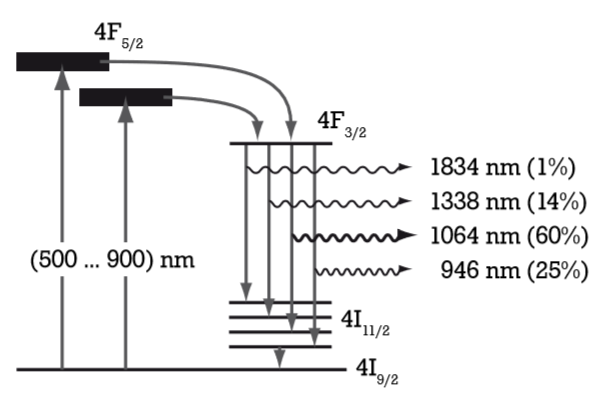
\includegraphics[width=\textwidth]{graphics/ndyagschem.PNG}
  	\label{ndschem}
   	\end{minipage}
\caption{Energienivauschema des Nd:YAG-Lasers}\cite{anl} 	
\end{figure}
Im Versuch wird eine Laserdiode zum optischen Pumpen des Nd:YAG Kristalls verwendet. Gepumpt wird der Laser aus dem $4I_{9/2}$ in die $4F_{6/2}$ Niveaus über Photonen mit einer Wellenlänge von $500\,\si{nm}<\lambda<900\,\si{nm}$, wobei folgende Wellenlängen mit hoher Effizienz gepumpt werden können:
\begin{align}
\lambda_{1}&=804,4\,\si{nm}\\
\lambda_{2}&=808,4\,\si{nm}\\
\lambda_{3}&=812,9\,\si{nm}\\
\lambda_{4}&=817,3\,\si{nm}\\
\end{align}
In diesem Bereich liegt auch die Emission des zum Pumpen verwendeten Diodenlasers, weshalb eine Kombination der beiden mit einer hohen Gesamteffizienz betrieben werden kann.\\
Von den oberen Pumpniveaus gehen die Elektronen nach einer kurzen Lebensdauer strahlungslos in den $4F_{3/2}$, das obere Laserniveau über. Dieser Zustand ist metastabil und besitzt aufgrund der verbotenen elektrischen Dipolstrahlung eine Lebensdauer von $240\,\si{\mu s}$. Vom oberen Lasernivau gibt es nun 4 Übergänge in das aufgespaltene untere Laserniveau, von denen vor allem der zu 60\% vorkommende Übergang in das $4I_{11/2}$ Niveau mit einer Wellenlänge von $\lambda=1064\,\si{nm}$ interessant ist. Dieser ist offensichtlich nicht im von Menschen sichtbaren Wellenlängen Bereich von $\approx 400\,\si{nm}\,-\,\approx 800\,\si{nm}$, lässt sich aber über die Frequenzverdopplung mittels eines KTP-Kristalles in Licht der Wellenlänge $\lambda=532\,\si{nm}$ konvertieren, welche im grünen Bereich des sichtbaren Spektrums liegt \ref{freq} \cite{anl,laser2,laser3}
\section{Nichtlineare Optik}
Phänomene der nichtlinearen Optik sind Konsequenzen der Modifikation der optischen Eigenschafte von Materialien bei der Anwesenheit von Licht. In der Regel besitzt nur Laserlicht ausreichend hohe Intensitäten, um die optischen Eigenschaften zu verändern. Die Phänomene werden als nichtlinear bezeichnet, da die Antwort auf das angelegte Feld, nichtlinear von der Intensität des Feldes abhängt. Betrachtet man die Abhängigkeit der Polarisation in der linearen konventionellen Optik, so ergibt sich, dass die Polarisation $\vec{P(t)}$ linear mit dem elektrischen Feld $\vec{E(t)}$ zusammenhängt. Die Relation ist über 
\begin{align*}
\vec{P(t)}=\varepsilon_0\chi^{(1)}\vec{E}(t)
\end{align*}
gegeben, wobei $\varepsilon_0$ die elektrische Feldkonstante bezeichnet und die Proportionalitätskonstante $\chi^{(1)}$ als elektrische Suszeptibilität bezeichnet wird. In der nichtlinearen Optik wird dieser Zusammenhang verallgemeinert und wird als Potenzreihe
\begin{align*}
\vec{P}(t)=\varepsilon_0 \left[ \chi^{(1)} \vec{E}(t) + \chi^{(2)} \vec{E}^2(t) +  \chi^{(3)}\vec{E}^3(t) + \dots \right]
\end{align*} 
dargestellt, wobei $\chi^{(2)}$ und $\chi^{(3)}$ als optische Suszeptibilitäten zweiter und dritter Ordnung bezeichnet werden. Dieser Zusammenhang, der voraussetzt, dass das Medium instantan antwortet, gilt jedoch nur unter Vernachlässigung von Absorption und Dispersion. Die Suszeptibilitäten hängen in der Regel noch von der Frequenz ab. Dabei beschreibt $\chi^{(1)}$ zum Beispiel Brechung und lineare Absorption, $\chi^{(2)}$ die Erzeugung der zweiten Harmonischen, das parametrische Mischen und die Erzeugung von Summen und Differenzfrequenzen und $\chi^{(3)}$ die Erzeugung der dritten Harmonischen, Raman- und Brillouin-Streuung und den Kerr-Effekt. [2,6]


\subsection{Frequenzverdopplung}\label{freq}
Bei der Frequenzverdopplung entsteht bei der Bestrahlung bestimmter Materialien mit Licht hoher Intensität Licht mit der doppelten Frequenz. Die elektromagnetische Strahlung regt im Material die Elektronen zum Schwingen an. Die Elektronen schwingen dabei mit der gleichen Frequenz wie die einfallende Strahlung, und erzeugen somit erneut elektromagnetische Strahlung. Bei hohen Intensität werden die Elektronen weiter ausgelenkt und die Rückstellkräfte sind nicht mehr proportional zur Auslenkung. Die dielektrische Polarisation des Materials ist nicht mehr linear vom elektrischen Feld abhängig, sondern es treten Terme höherer Ordnung auf. Dies führt dazu, dass die Polarisation außer der Frequenz der einfallenden Welle $\omega$ auch höhere Harmonische $m\cdot \omega$ ($m=2,3,4,...$) enthält. Die elektrischen Dipole strahlen daher auch elektromagnetische Wellen auf höheren Harmonischen ab. Die Erzeugung der zweiten Harmonischen resultiert aus dem Teil der atomaren Antwort, die quadratisch mit der Stärke des angelegten optischen Feldes zusammenhängt. Die Frequenzverdopplung, die Erzeugung der zweiten Harmonischen, wird wird auch als SHG (second harmonic generation) bezeichnet, die Frequenzverdreifachung als THG (third harmonic generation). 
Das elektrische Feld, welches durch
\begin{align*}
\vec{E}(t)=\vec{E}\cdot\text{e}^{-i\omega t} + c.c.
\end{align*}
repräsentiert wird, fällt auf einen Kristall dessen Suszeptibilität zweiter Ordnung nicht Null ist, und erzeugt die nichtlineare Polarisation zweiter Ordnung
\begin{align*}
\vec{P}^{(2)}(t)=2\epsilon_0\chi^{(2)}EE^*+\left(\epsilon_0\chi^{(2)}E^2\text{e}^{-i2\omega t}+c.c.\right)
\end{align*} 
Die Polarisation zweiter Ordnung setzt sich aus einem Term mit Frequenz Null und einem Term mit Frequenz $2\omega$ zusammen. Der zweite Beitrag erzeugt Strahlung mit der doppelten Frequenz, wohingegen der erste Term keine elektromagnetischer Strahlung erzeugt, sondern erzeugt ein statisches elektrisches Feld im Kristall (optische Gleichrichtung).
Anschaulich werden zwei Photonen der Frequenz $\omega$ zerstört und ein Photon der Frequenz $2\omega$ wird in einem einzelnen quantenmechanischen Prozess erzeugt. Die Frequenzverdopplung kann beispielsweise genutzt werden, um die Laserstrahlung des Nd:YAG-Lasers, der im nahen Infrarotbereich bei 1064 nm arbeitet, in den sichtbaren Spektralbereich bei 532 nm zu konvertieren. Von entscheidender Bedeutung für den Prozess der Frequenzverdopplung ist die Phasenanpassung. Die ursprüngliche Wellenlänge und die erzeugte doppelte Wellenlänge müssen im Kristall den gleichen Brechungsindex besitzen, da sonst destruktive Interferenz auftritt.
[2,6,7]	
\chapter{Versuchsdurchführung und Beobachtung}
  
     	
\chapter{Auswertung}
\chapter{Fazit}
\chapter{Messdaten}


\chapter{Anhang}





		

\renewcommand{\bibname}{Literatur}
\begin{thebibliography}{0}
\bibitem {prot1} Protokoll zum Versuch 4.4: Holographie, Tatjana Beynsberger und Dominik Pfeiffer 
\bibitem {anl} Anleitung zum Versuch 4.6, Version 1.6 (06.06.2013)
\bibitem {laser} Laser, F.K. Kneubühl und M.W. Sigrist, Teubner Verlag (Literaturmappe)
\bibitem {laser2} Anleitung zum Versuch 8 Nd:YAG-Laser, RTHW Aachen, Stand 12.03.2012
\bibitem {laser3} \url{www.laserschneiden-marktplatz.de/lasertypen/ndyag-laser} (Zugriff: 09.05.2017)
\bibitem {6} Robert W. Boyd: Nonlinear Optics. Elsevier Ltd, Oxford, 3. edition, 2008.
\bibitem {7} Literaturmappe im Anhang der Versuchsanleitung zum Versuch Hong-Ou-Mandel Effekt, TU Darmstadt
\bibitem {8} Hecht, Eugene: Optics, 4. Edition, 12 August 2001
\end{thebibliography} 	



\end{document} 